% ==================================================================
% APPENDIX A1 — Hubble + r_s: extraction of ε under uniform-ε def.
%
% FINAL DRAFT on freeze-checkpoint numbers (2026-04-19).
% Numerics: scripts/epsilon_convergence/ch1_hubble.py, result_ch1.json
% Background: scripts/epsilon_convergence/ect_background.py
% Figure:    scripts/fig_hubble_rs_extraction.py -> grayscale PDF
%
% Structure (unified per-probe template for A2-A5):
%   A1.1  Physics of the probe
%   A1.2  Observational inputs
%   A1.3  ECT-side model and extraction scope
%   A1.4  Extraction statistic
%   A1.5  Interval definition and origin of the width
%   A1.6  Figure
%   A1.7  Methodological limitations
%
% Applied corrections:
%   - GPT r16: H1-type framing upfront; no "resolves" language;
%     "held fixed / varied / not included" block; origin-of-width
%     paragraph; "why r_s matters physically" motivation.
%   - GPT r18/r19: no "ECT-native" overclaim; freeze-provisional
%     framing; t_0 treated as background quantity computed
%     self-consistently via ect_background; age-viability ambiguity
%     flagged as pending A6 interpretation (not asserted here).
%
% NO legacy numbers (3%, 0.010, 69 km/s/Mpc).
% NO integration into preprint yet — this is a frozen draft only.
% ==================================================================

\section{Extraction of the effective uniform-$\varepsilon$ interval
from the Hubble + $r_s$ channel}
\label{app:eps_extraction_hubble}

This appendix derives an effective H1-type extraction of
$\varepsilon$ from the simplified Hubble + $r_s$ channel used in the
rebuilt \S15.5. It is not a full CMB-to-local inference pipeline and
does not by itself establish a complete H2-level resolution of the
Hubble tension. Its output is the one-dimensional
$\varepsilon$-interval quoted for the Hubble + $r_s$ row of
Table~\ref{tab:eps_retained_probes_rebuilt}, extracted under the
uniform-$\varepsilon$ ansatz of \S\ref{subsec:eps_def_rebuilt} and
the common background module described in
Appendix~\ref{app:eps_methodology}. The forward-modelling machinery
--- the late-time ordered-branch background and its auxiliary
numerical algorithms --- is collected in
Appendix~\ref{app:late_cosmo_background} and
Appendix~\ref{app:late_cosmo_algorithm}. The present appendix is the
inverse step: given observational inputs and the uniform-$\varepsilon$
ansatz, to extract the one-dimensional $\varepsilon$-interval that
this single channel admits at the common-background level.

\subsection*{A1.1\quad Physics of the probe}

The Hubble tension is not simply a discrepancy between two direct
measurements of $H_0$: it is a mismatch between the local
distance-ladder value and the $H_0$ inferred from the acoustic
angular scale once the sound horizon $r_s$ is modelled. This is why
the present channel is naturally a Hubble + $r_s$ channel rather
than a pure $H_0$-only constraint. The local distance-ladder
determination $H_0^{\rm SH0ES}$ uses Cepheid-calibrated Type~Ia
supernovae and is insensitive to sound-horizon physics. The
CMB-based determination $H_0^{\rm Planck}$ is obtained from the
acoustic-scale angle $\theta_s = r_s / D_A(z_*)$, measured to high
precision by the Planck mission~\cite{Planck2018}. A shift in the
inferred late-time expansion rate arises once the late-time
gravitational response function is allowed to differ from the
$\Lambda$CDM form. In the effective uniform-$\varepsilon$ layer of
\S\ref{subsec:eps_def_rebuilt} this response is parametrised by
\begin{equation}
\frac{G_{\rm eff}(z)}{G_N} \;=\; (1+z)^{2\varepsilon}.
\label{eq:Geff_uniform_eps_A1}
\end{equation}
Under this parametrisation, both the low-redshift distance integral
(entering $H_0^{\rm Planck}$ through $D_A(z_*)$) and the high-redshift
sound-horizon integral (entering $r_s$) are modified. The channel
therefore tests $\varepsilon$ through the joint constraint imposed
by a fixed, precisely measured $\theta_s$ and an independently
determined local $H_0$. The output of the extraction is an H1-type
effective band for $\varepsilon$: a range of values for which the
common-background module, deformed by $(1+z)^{2\varepsilon}$,
shifts the CMB-inferred $H_0$ upward into statistical compatibility
with the local distance-ladder value.

\subsection*{A1.2\quad Observational inputs}

The two anchoring values are
$H_0^{\rm Planck} = 67.4 \pm 0.5~\mathrm{km\,s^{-1}\,Mpc^{-1}}$
from Planck~2018 in $\Lambda$CDM~\cite{Planck2018} and
$H_0^{\rm SH0ES} = 73.04 \pm 1.04~\mathrm{km\,s^{-1}\,Mpc^{-1}}$
from the SH0ES distance-ladder analysis~\cite{Riess2022}. The target
shift to be accommodated is therefore
\begin{equation}
\Delta H_0^{\rm obs}
\;\equiv\; H_0^{\rm SH0ES} - H_0^{\rm Planck}
\;\approx\; 5.64~\mathrm{km\,s^{-1}\,Mpc^{-1}},
\qquad
\sigma_{\rm tot} \;=\; \sqrt{\sigma_P^2 + \sigma_{\rm SH}^2}
\;\approx\; 1.15~\mathrm{km\,s^{-1}\,Mpc^{-1}}.
\end{equation}
The acoustic-scale measurement $\theta_s$ is taken as fixed at the
Planck value; the $\varepsilon$-scan is carried out at fixed
$\theta_s$, such that the $\varepsilon$-deformation modifies $r_s$
and $D_A(z_*)$ in correlated ways.

\subsection*{A1.3\quad ECT-side model and extraction scope}

Under the uniform-$\varepsilon$ ansatz, the dimensionless Hubble rate
reads
\begin{equation}
E_{\rm ECT}^2(z,\varepsilon)
\;=\; \Omega_r\,(1+z)^4
\;+\; \Omega_m\,(1+z)^{3+2\varepsilon}
\;+\; \Omega_\Lambda\,(1+z)^{2\varepsilon},
\label{eq:eps_friedmann_A1}
\end{equation}
with $\Omega_m = 0.315$, $\Omega_r = 9.2 \times 10^{-5}$,
$\Omega_\Lambda = 1 - \Omega_m - \Omega_r$ adopted as the common
background proxy (see Appendix~\ref{app:eps_methodology} for the
background-module framing and its role as the single source of
truth for all retained extraction channels). The low-redshift
distance integral is
\begin{equation}
I(\varepsilon) \;=\; \int_0^{z_*}
\frac{dz}{E_{\rm ECT}(z,\varepsilon)},
\qquad z_* = 1089.80,
\end{equation}
and the sound horizon at the drag epoch is
\begin{equation}
r_s(\varepsilon)
\;=\; \int_{z_{\rm drag}}^{\infty}
\frac{c_s(z)}{H_0^P\,E_{\rm ECT}(z,\varepsilon)}\,dz,
\qquad z_{\rm drag} = 1059.94,
\end{equation}
with the baryon--photon sound speed
$c_s(z) = c/\sqrt{3(1+R(z))}$,
$R(z) = (3\Omega_b / 4\Omega_r)(1+z)^{-1}$, $\Omega_b = 0.0493$.
At fixed $\theta_s$, the inferred $H_0$ under
$\varepsilon$-deformation becomes
\begin{equation}
H_0^{\rm inferred}(\varepsilon)
\;=\; H_0^P \cdot
\frac{I(\varepsilon)}{I(0)}
\cdot
\frac{r_s(0)}{r_s(\varepsilon)}.
\label{eq:H0_inferred_eps}
\end{equation}
For $\varepsilon > 0$, the sound-horizon integral decreases by a
larger fractional amount than the distance integral, so the ratio
in \eqref{eq:H0_inferred_eps} exceeds unity and $H_0^{\rm inferred}$
is pushed upward.

\paragraph{Held fixed under the present proxy.}
$\Omega_m = 0.315$, $\Omega_\Lambda$, $\Omega_r$, $\Omega_b$; the
baryon--photon sound-speed form $c_s(z)$; $z_* = 1089.80$,
$z_{\rm drag} = 1059.94$; the acoustic-scale anchor $\theta_s$.

\paragraph{Varied.}
$\varepsilon$ only (one-dimensional scan). Through
\eqref{eq:eps_friedmann_A1} the variation of $\varepsilon$
propagates automatically, via the common background module, into
$E(z)$, $H(z)$, $I(\varepsilon)$, $r_s(\varepsilon)$, and
$H_0^{\rm inferred}(\varepsilon)$.

\paragraph{Not included at this proxy level.}
A full Boltzmann-level recombination pipeline; a full CMB
likelihood; a joint fit of early-time parameters together with
$\varepsilon$; and an ECT-closure-level background replacing the
$\Lambda$CDM proxy. The consequences of each of these omissions
are addressed in A1.7.

\subsection*{A1.4\quad Extraction statistic}

The $\varepsilon$-dependent prediction for the Hubble-tension shift
is
\begin{equation}
\Delta H_0^{\rm pred}(\varepsilon)
\;=\; H_0^{\rm inferred}(\varepsilon) - H_0^P.
\end{equation}
The single-parameter chi-squared for this channel is
\begin{equation}
\chi^2(\varepsilon)
\;=\;
\left[\,
\frac{\Delta H_0^{\rm pred}(\varepsilon) - \Delta H_0^{\rm obs}}
     {\sigma_{\rm tot}}
\,\right]^{\!2}.
\label{eq:chi2_hubble_eps}
\end{equation}
This is the only quantity minimised in the present extraction; no
additional nuisance-parameter profiling is performed at this proxy
level.

\subsection*{A1.5\quad Interval definition and origin of the width}

In this one-parameter framework the best-fit $\varepsilon_*$ is
defined by the minimum of $\chi^2(\varepsilon)$, which coincides
with the unique root of $\Delta H_0^{\rm pred}(\varepsilon) =
\Delta H_0^{\rm obs}$ in the physical region $\varepsilon \geq 0$.
The $1\sigma$ interval is defined by $\Delta\chi^2 \leq 1$ about
this minimum, the $2\sigma$ interval by $\Delta\chi^2 \leq 4$.
Both are obtained by Brent root-finding on the equivalent
conditions
$\Delta H_0^{\rm pred}(\varepsilon) =
\Delta H_0^{\rm obs} \pm \sigma_{\rm tot}$
and
$\Delta H_0^{\rm pred}(\varepsilon) =
\Delta H_0^{\rm obs} \pm 2\sigma_{\rm tot}$.

\paragraph{Origin of the $1\sigma$ width.}
The width of the $1\sigma$ interval is determined by the curvature
of the one-parameter profile $\chi^2(\varepsilon)$ around its
minimum under the adopted observational uncertainty
$\sigma_{\rm tot}$. It therefore reflects the uncertainty of the
present proxy extraction of $\varepsilon$ from the adopted
observational inputs, not a first-principles uncertainty of the
ECT closure parameters. A narrower or wider $\sigma_{\rm tot}$
would shrink or widen the interval accordingly; a fundamentally
different proxy setup, or a full ECT-closure-level background
replacing the common proxy of A1.3, would in general reshape both
the location and the width of the interval.

\paragraph{Numerical outcome.}
Direct numerical evaluation of the integrals in A1.3 through the
common background module
(\texttt{ect\_background.py}, consumed by
\texttt{ch1\_hubble.py}) yields
\begin{align}
\varepsilon_*
&\;=\; 0.0323,
\label{eq:eps_hubble_central}
\\[2pt]
[\varepsilon_{\rm lo}^{1\sigma},\,\varepsilon_{\rm hi}^{1\sigma}]
&\;=\; [\,0.0267,\ 0.0376\,],
\\[2pt]
[\varepsilon_{\rm lo}^{2\sigma},\,\varepsilon_{\rm hi}^{2\sigma}]
&\;=\; [\,0.0207,\ 0.0425\,].
\end{align}
The $1\sigma$ width $\Delta\varepsilon^{1\sigma} \approx 0.0109$
inherits approximately linearly from $\sigma_{\rm tot}$. This is
the numerical content of the Hubble + $r_s$ row of
Table~\ref{tab:eps_retained_probes_rebuilt} in
\S\ref{subsec:eps_retained_rebuilt}.

\paragraph{Background-level cosmic age at the extracted
$\varepsilon_*$.}
Computed through the same common background module, the
age-of-universe at the Hubble best-fit is
$t_0(\varepsilon_* = 0.0323) \approx 13.46~{\rm Gyr}$, compared
with $t_0(\varepsilon = 0) \approx 13.79~{\rm Gyr}$ at the
$\Lambda$CDM baseline. The role of this quantity --- and the
distinction between the background cosmic age at fixed baseline
$H_0^P$ and the age under the inferred-$H_0$ mapping of
\eqref{eq:H0_inferred_eps} --- is discussed in
Appendix~\ref{app:eps_methodology} as an age-viability ambiguity,
and is not used as an independent $\varepsilon$-constraint here.

\subsection*{A1.6\quad Figure}

\begin{figure}[H]
\centering
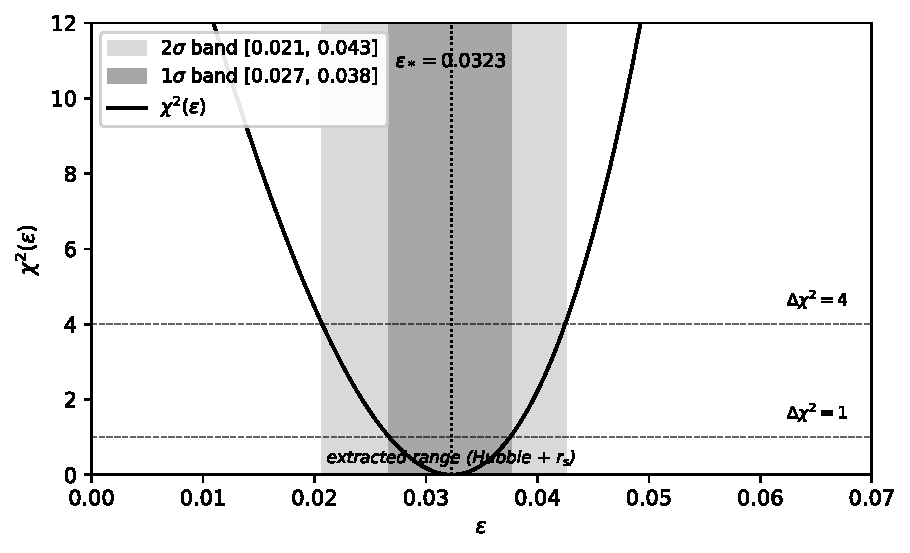
\includegraphics[width=0.82\textwidth]{figures/fig_hubble_rs_extraction_bw.pdf}
\caption{Extraction of the effective $\varepsilon$-interval from the
Hubble + $r_s$ channel, under the common background module of
Appendix~\ref{app:eps_methodology}. The solid black curve is
$\chi^2(\varepsilon)$ defined by \eqref{eq:chi2_hubble_eps}. The
darker gray band is the $1\sigma$ interval $[0.027,\,0.038]$
($\Delta\chi^2 \leq 1$); the lighter gray band is the $2\sigma$
interval $[0.021,\,0.043]$ ($\Delta\chi^2 \leq 4$). The dotted
vertical line marks the best-fit
$\varepsilon_* \approx 0.0323$. Horizontal dashed lines indicate
the $\Delta\chi^2 = 1$ and $\Delta\chi^2 = 4$ reference levels.
All shading and line styles are grayscale per preprint
convention.}
\label{fig:hubble_rs_extraction}
\end{figure}

\subsection*{A1.7\quad Methodological limitations}

Four limitations are stated explicitly. The first three are
inherited by every other per-probe extraction appendix of this
family; the fourth is more specific.

\textit{(i) $\Lambda$CDM-background common proxy.}
The common background module uses a $\Lambda$CDM-best-fit
parameter set as external input, and the $\varepsilon$-deformation
is applied on top. A fully ECT-closure-level extraction would
replace this proxy by the derived ordered-branch background of
Appendix~\ref{app:late_cosmo_background} rather than a fit
obtained under a different theoretical assumption set.

\textit{(ii) Simplified sound-horizon integral.}
The sound-horizon integral is computed with a simplified
baryon--photon sound speed $c_s(z)$, a $z_{\rm drag} = 1059.94$
anchor, and neutrino effects absorbed into $\Omega_r$. At the
level of the absolute $r_s$ this introduces a few-per-cent
discrepancy with the Planck~2018 value; however, only the ratio
$r_s(\varepsilon) / r_s(0)$ enters the extraction
\eqref{eq:H0_inferred_eps}, and this ratio is more robust than
either absolute value.

\textit{(iii) Uniform-$\varepsilon$ ansatz vs closure-level
$\varepsilon(z)$.}
The uniform-$\varepsilon$ ansatz treats $\varepsilon$ as
epoch-independent. A first-principles $\varepsilon(z)$ from
three-stage condensate closure --- the content of OP-Hubble-derive
(\S\ref{subsec:eps_outlook_rebuilt}) --- would reshape the width
of the retained interval and in general would not map one-to-one
onto a constant $\varepsilon$. The retained interval derived here
should therefore be read as the projection of the true
$\varepsilon(z)$ history onto the uniform-$\varepsilon$
diagnostic layer, not as a measurement of a fundamental constant.

\textit{(iv) Age--$H_0$ mapping is not fixed by this channel.}
The background module computes $t_0(\varepsilon)$
self-consistently. However, the physical interpretation of the
cosmic age at the extracted $\varepsilon_*$ depends on which of
two mappings is adopted: (a) the baseline-background age at fixed
$H_0^P = 67.4~\mathrm{km\,s^{-1}\,Mpc^{-1}}$, which is acceptable
with respect to direct age anchors; or (b) the age under the
inferred-$H_0^{\rm inferred}(\varepsilon_*)$ mapping
\eqref{eq:H0_inferred_eps}, which is more sensitive to the same
anchors. Nothing in the Hubble + $r_s$ channel alone discriminates
between these two mappings: the channel determines $\varepsilon_*$
only via $\theta_s$-preservation. The interpretation of this
ambiguity and its implications are discussed as the age-viability
ambiguity in Appendix~\ref{app:eps_methodology}; this appendix
does not use the cosmic age as an independent constraint on
$\varepsilon$.

% ==================================================================
% END Appendix (extraction, Hubble + r_s channel).
% ==================================================================
